\documentclass[10pt]{article}
\usepackage[a4paper,margin=20mm]{geometry}
\usepackage[T1]{fontenc}
\usepackage{lmodern,microtype,amsmath,amssymb,graphicx,booktabs,longtable,array,tabularx}
\usepackage[super,sort&compress]{natbib}
\usepackage{hyperref}
\hypersetup{colorlinks=true,urlcolor=blue,citecolor=blue,linkcolor=blue,pdftitle={Supplement: Choosing scientific visualizations through task-first optimization},pdfauthor={Mohamed Elgendi}}
\setlength{\parindent}{0pt}\setlength{\parskip}{5pt}\emergencystretch=4em
\title{Supplementary information\\Choosing scientific visualizations through task-first optimization}
\author{Mohamed Elgendi}\date{}
\renewcommand{\thefigure}{S\arabic{figure}}
\renewcommand{\thetable}{S\arabic{table}}
\begin{document}\maketitle
\section*{S1. Scope and evidence map}
The primary study evaluates six tasks: median, spread, five distributional gaps, composition, ordered profiles and correlation. The empirical task count is $3\times127+24+72+53=530$. The new synthetic evaluation contributes $3\times36+48+36+36=228$ task instances. Reused inputs and task instances must not be counted as independent biological observations.

Primary results are in \texttt{benchmark\_release/results/}. Marginal rendering and recovery are implemented in \texttt{validation\_v3/} and its explicitly retained lower-level dependencies. Composition, profile and association implementations are in \texttt{task\_first/}. These directory names identify software modules, not separate submitted manuscript versions. Raw and prepared inputs, complete trial outputs and historical sensitivity analyses are retained. The main manuscript and this Supplement are the current scientific narrative; archived manuscripts are provenance only. Main Figures 1, 2 and 4 retain the familiar-chart teaching displays, while Figures 3, 5 and 6 report the full strong-default, decoder and synthetic analyses.

The primary marginal candidate set has ten fixed configurations: seven familiar families, one ECDF and two explicit quantile-marker configurations. The broader task implementations comprise 13 familiar families. No worldwide popularity ranking is claimed. The additional distributional controls are intentionally included even though they are less familiar. Families without an implemented task contract are not assigned zero scores.

The earlier 21-setting familiar-family search and 23-setting expanded search are secondary tuning-budget analyses. Their counts and outcomes are not pooled with the fixed-setting primary comparisons. No human-reader data or new clinical cohorts are included.

\section*{S2. Fixed familiar rendering and hard-color recovery}
The retained renderer supports the full settings below. The primary fixed candidate set uses raw dots, 16-bin histograms and heatmaps, and 64-point violins; mean dots and other bin/grid settings belong only to the secondary tuning-budget audit.

\textbf{Target.} NumPy's default linear empirical quantiles at probabilities $(.1,.25,.5,.75,.9)$ define five equally weighted differences, group B minus group A. The target is descriptive and marginal even when the source observations are paired. It is not a full-distribution metric or an estimate of individual change.

\textbf{Normalization.} Pooled within-group standard deviation weights each sample variance by its degrees of freedom. If that standard deviation is zero, the implementation uses one source unit and records a fallback flag. This special case is not unit-invariant. All eligible candidates within a comparison share the same scale.

\textbf{Range.} Let $h_g=\mathrm{SD}(g)n_g^{-1/5}$ and $b=\max(h_x,h_y,.01s)$. The measurement range is $[\min(0,\min(x,y)-4b),\max(0,\max(x,y)+4b)]$. If needed, a degenerate upper limit is replaced by the lower limit plus one. All families use this range, including histogram and heatmap bins. Zero inclusion supports bars but may reduce useful resolution for other displays; it is an explicit design limitation.

\textbf{Inputs to the decoder.} RGB image, family, setting, panel resolution, image width, measurement limits, panel bounding coordinates and declared group colours. The decoder is not given samples, target quantiles, pre-rendered summary values, placement offset or jitter seed. It is given exact axes rather than recovering tick labels through optical character recognition. The chart type is known.

\textbf{Raster geometry.} Two panels of side $H\in\{128,256,512\}$ are separated by 16 pixels. Each plotting region extends from local horizontal coordinate 8 to $H-9$ and vertical coordinate 8 to $H-9$. RGB colours are $(38,126,165)$ and $(223,120,54)$. Images are first drawn at fourfold resolution, reduced with Lanczos filtering and blurred by a Gaussian radius of 0.5 target pixels. Measurement marks use vertical offsets 0, .25, .5 and .75 pixels. These placements are sensitivity conditions, not independent samples of reader performance.

\textbf{Bars and dots.} Mean bars have width $0.4H$ and extend from zero to the group mean. Mean dots have radius two target pixels. Raw dots have radius 1.5 pixels and uniformly jittered horizontal centres within $\pm0.35H$ of the panel centre. Random seeds are $20260920+r+100003g$, with zero-based placement index $r$ and group index $g$. Thus raw-dot realizations vary both placement and jitter. The dots are opaque; within-group overlaps are retained.

\textbf{Boxes and intervals.} A one-pixel minimum--maximum line is common to both. A box has width $0.4H$ and spans the interquartile range, with a one-pixel black median line. The interval has a five-pixel interquartile line and black median marker of radius 2.5 pixels. These are five-number summaries of observations, not standard errors, confidence intervals or Tukey outlier conventions.

\textbf{Histograms and heatmaps.} Bin counts $4,8,16,32,64$ share equal-width measurement bins. Histogram heights represent group probabilities on a fixed zero-to-one axis. Heatmap tiles encode probability $m$ as $(\mathrm{round}(255(1-m)),\mathrm{round}(255(1-m)),255)$. The heatmap strip occupies the middle 30\% of plot height; its raster is invariant across the four vertical placements. This known linear colour scale is an oracle supplied through the implemented decoder, not evidence of perceptual linearity.

\textbf{Violins.} Group-specific Gaussian kernel densities use SciPy's Scott bandwidth and are sampled on common grids of $8,16,32,64,128,256$ points. Width is normalized separately by each group's peak to $0.4H$. The rendered polygon connects those grid points; no finer smoothing is inserted into the displayed figures. Constant samples use a Gaussian width of $.01s$, evaluated with a stabilized exponential to avoid underflow.

\textbf{Pixel extraction.} A pixel is group-coloured if its Euclidean RGB distance from the known group colour is below 80. A black mark has RGB norm below $.78$ times the group-colour norm. Bars use rows with coloured width exceeding 20\% of plot width, taking the endpoint farther from zero. Mean dots use the coloured row-mass centroid. Box and interval extrema use any coloured or black mark; interquartile bounds use row width above 30\% of plot width for boxes or 2.5 pixels for intervals. Median position is the black row-mass centroid. Recovered five-number landmarks are monotonized and linearly interpolated to the target probabilities.

Histogram probabilities come from the top coloured pixel at each bin-centre column relative to the known baseline. Heatmap probabilities come from inverse red intensity at tile centres. Negative recovered masses are clamped to zero and masses normalized. Their cumulative inverse uses linear interpolation within each nonempty bin. Violin and raw-dot decoders instead invert cumulative coloured pixel area by measurement row. This is an area-based observer, not a point-counting algorithm or an optimal image decoder. Empty recoveries fail explicitly.

\textbf{Score and optimization.} For each realization, divide mean absolute contrast error by the shared scale. Average that loss over all four realizations, then transform by $100/(1+L)$. Do not average scores before optimization. A setting with any failed realization is excluded. Within each family select its lowest mean loss; ties can be displayed deterministically but remain equal scientific outcomes. Across families, absolute loss differences at most $10^{-12}$ are treated as ties, with no relative tolerance. Unrounded values determine rankings. Displaying three decimals does not assert precision or practical significance.


\section*{S3. Distributional controls and the soft-color observer}
\textbf{ECDF.} Sort each group's observations. At every observation, draw the horizontal cumulative-probability step from $i/n$ to $(i+1)/n$, with measurement mapped to vertical position; join steps vertically and extend to the declared measurement bounds. The stroke is two target pixels wide. This is the ordinary empirical cumulative step function with axes transposed, not a smoothed density. For each requested probability, read the colored pixel column and estimate its vertical centroid. Finite-pixel vertical segments and the difference between the ECDF inverse and linear-interpolated sample quantiles can generate error.

\textbf{Quantile plot.} Render five colored markers with radius two target pixels at horizontal positions $p_k$ and vertical positions $Q_g(p_k)$. Read a five-column window around each target probability and calculate the vertical pixel-mass centroid. The decoder receives the declared probability locations, which are task metadata shared across all comparisons, but no numerical quantile values. Monotonize the recovered sequence with a cumulative maximum. A display constructed from task-relevant summaries is allowed; transferring those summaries to the decoder as numerical metadata is not.

\textbf{Alpha observer.} For RGB pixel $a$ and known group color $c$, compute
\[
\alpha(a)=\operatorname{clip}_{[0,1]}\left\{\frac{(255-a)\cdot(255-c)}{\|255-c\|^2}\right\}.
\]
Geometric masks use $\alpha>0.2$. Integrated row mass sums $\alpha$ only where it exceeds 0.05. Bar, mean-dot, box, interval, histogram, raw-dot and violin recovery otherwise follow the declared geometric contracts. Black median detection retains the original threshold. Heatmaps instead average the red channel over a local $3\times3$ neighborhood before inversion. The added ECDF and quantile plots use projected ink above 0.05 for their column or window centroids. The original observer uses the RGB-distance mask.

This observer is an alternative implementation, not an optimal decoder, an independent laboratory replication or a validated human model. It shares axis calibration, chart knowledge and much geometry with the original. The analysis evaluates sensitivity to specified extraction choices, not robustness to all possible readers.

\section*{S4. Mathematical interpretation and information limits}
For finite nonnegative loss, $0<S\leq100$. The reciprocal transformation preserves the complete loss ordering and all ties. A logarithmic transformation would also preserve ties. There is no valid mathematical reason to inject chart-specific offsets solely to create distinct ranks.

\textbf{Shared-error cancellation.} Let $e_{g,k}=\widetilde Q_g(p_k)-Q_g(p_k)$. Group-level loss averages absolute errors across both groups:
\[G=\frac{1}{10s}\sum_{g\in\{x,y\}}\sum_{k=1}^{5}|e_{g,k}|.\]
Contrast error is $e_{y,k}-e_{x,k}$, so the triangle inequality yields $L\leq2G$. If $e_{y,k}=e_{x,k}=b$ for every $k$, contrast loss is zero but group loss is $|b|/s$. Therefore a high contrast score cannot certify faithful recovery of either distribution. Both quantities are retained.

\textbf{A mean-only identifiability limit.} Consider a common fixed axis, equal group sample sizes and
\[
 x=(2,2,4,4),\quad y^{(1)}=x,\quad y^{(2)}=(3-\sqrt2,3,3,3+\sqrt2).
\]
Every group has mean 3 and sample variance $4/3$. Thus the mean-only images and calibration can be identical in the two scenarios, while their quantile-contrast vectors differ. The common scale is $s=\sqrt{4/3}$. If a decoder returns the same contrast vector $z$ for those identical inputs, then
\[
 \max\!\left\{\frac{\|z-\Delta^{(1)}\|_1}{5s},\frac{\|z-\Delta^{(2)}\|_1}{5s}\right\}
 \geq \frac{\|\Delta^{(1)}-\Delta^{(2)}\|_1}{10s}>0.
\]
This elementary bound concerns information omitted by the mean summary. The common fixed axis is essential: data-dependent axes could otherwise transmit extra information. The construction does not claim that every mean-bar rendering is poor or that its numerical lower bound applies to the benchmark's adaptive axes.

\textbf{Empirical versus population target.} For population contrast $\Delta^{\mathrm{pop}}$,
\[
\frac15\sum_k|\widetilde\Delta_k-\Delta^{\mathrm{pop}}_k|
\leq\frac15\sum_k|\widetilde\Delta_k-\Delta_k|+\frac15\sum_k|\Delta_k-\Delta^{\mathrm{pop}}_k|.
\]
The benchmark evaluates the first term. It does not provide confidence coverage for the second. Resolution sensitivity is not sampling uncertainty.

\textbf{Scale and translation.} For nonconstant samples, positive unit scaling multiplies the range, target, recovered values and normalization together. Fixture checks verify this behavior. Zero-inclusive axes are not translation invariant. Tight axes remove the zero inclusion but retain the four-bandwidth padding. Bars are excluded from both sides of that sensitivity. A different positive normalizer shared by every candidate for one comparison cannot change its loss ordering, but can change cross-comparison summaries. The constant-scale fallback is explicitly source-unit dependent.

\section*{S5. Nineteen-marker control and task extraction}
The nineteen-marker control places a radius-two marker at each empirical quantile $p=.05,.10,\ldots,.95$ in each group. The measurement axis and rendering operations match the five-marker control. The hard and soft observers integrate recovered ink within a five-column window around each known probability position. Recovered quantiles are monotonized. The calibration supplies marker probability positions and axis limits, never the numerical quantiles.

For the primary tasks, the two groups' recovered quantiles determine the median difference, difference of interquartile ranges and gaps at $.1,.25,.5,.75,.9$. The five-marker control interpolates between its specified probability positions where another task needs additional quantiles. Nineteen markers have more encoding capacity; they are disclosed as a distinct configuration rather than treated as an equal mark-budget implementation. Primary candidate settings are fixed; no family-specific tuning is conducted in the main comparisons.

Three additional marginal tasks remain in the electronic sensitivity results: tail asymmetry, upper-tail extent and nineteen quantile gaps. They do not add independent input cases. Their definitions and complete recovery outputs are in \texttt{validation\_v3/benchmark.py} and \texttt{decoded\_trials.csv}.

\section*{S6. Composition, profile and association contracts}
\textbf{Composition inputs.} Pooled quartiles of the first canonical feature in each resource define four categories. The two groups produce 18 empirical share vectors. The valid group counts in the six unpaired resources give six binary cohort compositions. All categories remain present, including zero-count bins. These transformations change a continuous-data question into a category-share question and are explicitly recorded. The 48 earlier synthetic compositions use Dirichlet draws at four category counts and three concentration parameters. They are separate from the 48 newly generated compositions used in the final transfer study.

\textbf{Profile inputs.} Positive finite heart-rate measurements from each source recording are divided into twelve equal-duration bins and averaged. No bin is empty and no retained empirical profile has zero SD. Wrist profiles use 19 recordings from eight participants; BIDMC uses 53 recordings from 46 patients. The target is the twelve means, not a continuous-time trajectory or a clinical trend diagnosis. The rendering implementation supports nonnegative profiles and shares a zero-origin scale across candidates. Profiles with a small SD can have large normalized error even when absolute heart-rate error is small.

\textbf{Association inputs.} Positive finite ECG-HR and pulse pairs are systematically reduced to at most 64 equally spaced rows within each BIDMC recording. Targets refer to Pearson correlation of the displayed subset. This is not agreement, interchangeability or causal association. Repeated source recordings retain their patient identifiers for default training and uncertainty calculations.

\textbf{Rendering.} New-task panels are square. With $H$ pixels, plotting boundaries are $L=T=12$ and $R=B=H-13$. The eight-color palette is fixed in \texttt{task\_first/benchmark.py}. Composition bars use equal widths, pies fill a fixed-radius circle, donuts remove an inner radius of 52\%, and stacked bars share one horizontal baseline. Profiles use two-pixel lines, filled polygons, radius-two dots or equal-width bars. Scatter plots use radius-two opaque marks. Association heatmaps use a $16\times16$ probability grid and the declared linear white-to-blue encoding. Fourfold supersampling, Lanczos reduction and 0.5-pixel blur match the marginal renderer.

\textbf{Original composition readers.} The hard observer assigns non-white pixels to the nearest declared palette color and retains assignments with Euclidean RGB distance below 80. The soft observer weights assignments by their projected color opacity. Category masses are normalized to sum to one. A blank image fails. These operations count rendered colored area, not perceived angles or bar lengths.

\textbf{Original profile readers.} At twelve public horizontal positions, line and dot values are recovered from vertical ink centroids. Filled areas and bars use the top recovered boundary. The hard observer uses the color threshold; the soft observer uses projected ink. Known axes convert pixel coordinates to values. Missing values invalidate the rendering.

\textbf{Original association readers.} Scatter recovery computes weighted correlation from the coordinates of colored pixel mass, with vertical coordinates reversed. Opaque overlap can reduce represented multiplicity. Heatmap recovery inverts the red channel at bin centers; the soft reader averages a local $3\times3$ patch. The resulting cell masses determine correlation. No source pairs are supplied to either reader.

\section*{S7. Strong defaults, transfer and dependence}
Default selection and case-specific selection both use reference conditions only: 256-pixel panels and four phases $0,.25,.5,.75$. Test conditions use 384-pixel panels and phases $.125,.375,.625,.875$. This changes resolution and placement jointly. Four losses are averaged before score conversion. Any failed phase invalidates a candidate in that condition.

For median, spread, five-gap and composition tasks, each held-out resource is excluded when learning the default. Training losses average within resource and then across resources. For profiles, repeated recordings first average within source participant; the held-out source is excluded completely. Only BIDMC and wrist sources are available for this task. For association, every recording of the held-out patient is excluded, and training losses weight patients equally. A candidate must decode every training case to qualify as a learned default. The chosen default minimizes the resulting mean loss, with the same numerical tie tolerance as case-specific selection.

Case-specific selection minimizes that case's reference loss. It is allowed to use source data to evaluate the numerical target at the reference condition; it is not a learned recommender that predicts a chart without rendering the alternatives. The source observations are withheld from the decoder, not from the evaluator. This distinction is important for interpreting the method and its computational cost.

The scientific winning set includes all candidates within absolute loss tolerance $10^{-12}$ of the minimum. A fixed candidate order chooses a representative only for deployment. That order is listed in \texttt{benchmark\_release/common.py}. Exact computational ties are retained. No human-equivalence threshold is inferred from numerical tolerance.

Transfer loss is read from the frozen candidate's test-display result. The later-display minimum is a hindsight comparator and is never used to select the deployed chart. A default or selection failure is reported rather than replaced by a favorable number. Paired means use cases where both policies are valid; default and selected failures remain separate.

\begin{longtable}{llrrrrr}
\caption{Case-specific selection versus strong defaults on empirical data.}\label{tab:policy-outcomes}\\
\toprule Task & Reader & Cases & Sources$^*$ & Better & Worse & Tied\\\midrule\endhead
Median difference & hard & 127 & 9 & 31 & 41 & 55\\
Median difference & soft & 127 & 9 & 30 & 43 & 54\\
Spread difference & hard & 127 & 9 & 22 & 28 & 77\\
Spread difference & soft & 127 & 9 & 21 & 26 & 80\\
Five distributional gaps & hard & 127 & 9 & 7 & 10 & 110\\
Five distributional gaps & soft & 127 & 9 & 9 & 13 & 105\\
Category shares & hard & 24 & 9 & 4 & 4 & 16\\
Category shares & soft & 24 & 9 & 2 & 1 & 21\\
Ordered profile & hard & 72 & 2 & 0 & 6 & 66\\
Ordered profile & soft & 72 & 2 & 0 & 0 & 72\\
Correlation & hard & 53 & 46 & 5 & 4 & 44\\
Correlation & soft & 53 & 46 & 11 & 0 & 42\\
\bottomrule\end{longtable}
\noindent $^*$Sources are the resampling units; for correlation, the 46 units are patients. ``Better'' and ``Worse'' refer to case-specific selection relative to the strong default; ``Tied'' means an absolute error difference of at most $10^{-12}$. Hard and soft denote Reader 1 and Reader 2 in the main figures. Counts describe cases and do not imply independence. All 1,060 empirical case--reader policy pairs were successfully decoded: neither the default nor the selected policy failed. This does not mean that every candidate decoded successfully; candidate-level failures remain in the electronic results and are reported separately for the synthetic evaluation below.

The nine resource means or 46 association-patient means are resampled with replacement 5,000 times using seed 2026092202. Percentile limits are descriptive. The two profile-source means are reported without a bootstrap interval. Point estimates are not weighted by the number of features contributed by a resource. There is no pooled task score, simultaneous confidence statement or claim of equivalence based on an interval containing zero.

\section*{S8. Separate geometry reader}
The geometry decoder in \texttt{benchmark\_release/geometry\_observer.py} was implemented separately from colored-area recovery. For pie and donut charts, it samples 4,096 uniformly spaced angular positions at 76\% of the nominal outer radius about the public center. Pixels are assigned to the nearest declared category color if their RGB distance is below 80. Category shares are proportions of retained angular assignments. The known center does not include the hidden subpixel phase.

For bars, the decoder reads each category's center column, finds its highest recognized pixel and converts that endpoint to a height using the public baseline. Heights are normalized across categories. For stacked bars, it counts category assignments along the public central horizontal scanline. Zero-height categories may have no recovered pixels and are retained at zero; an entirely blank recovery fails. The public calibration contains geometry and colors but no true proportions.

The analysis covers all 24 empirical and 48 earlier synthetic compositions, four families, two display sizes and four placements: 2,304 decoder evaluations. Each family passes a known-proportion fixture and rejects blank images. Every trial in this analysis succeeds. This decoder changes the mechanism but shares the author, renderer and calibration assumptions. It is not an external replication. Geometry output is retained at full precision, including ties and decoder disagreements.

\section*{S9. New synthetic inputs and frozen defaults}
New synthetic inputs use seed 2026092201. The full generator and saved inputs are included. Before rendering them, one default per task and observer is frozen using all empirical reference conditions with the same resource/participant weighting as the primary analysis. These fixed empirical-trained defaults are: interval display for the hard median task; nineteen markers for the soft median task; five markers for both spread and five-gap tasks; pies for composition; dots for profiles; and heatmaps for association.

\textbf{Two groups.} Six regimes, two equal-group sample sizes ($30,150$) and three replicates produce 36 inputs. Regimes are independent standard-normal groups; a 0.5-SD location shift; a scale increase to 1.8; lognormal groups with log-SDs 0.5 and 1; a standard normal versus an equally weighted mixture centered at $-1.5$ and $1.5$ with within-component SD 0.4; and $t_3$ versus $0.3+1.3t_3$. A null generating process does not force a zero empirical difference.

\textbf{Composition.} Category counts $2,3,5,8$, symmetric Dirichlet concentrations $0.3,1,5$ and four replicates produce 48 share vectors. These are new draws, separate from the earlier seed-20260921 sensitivity set.

\textbf{Profiles.} Twelve positions span $[0,1]$. Shapes are a ramp, one sine-wave cycle or a step at 0.5. Relative amplitudes $0.01,0.1,0.4$ and four replicates give 36 profiles. Each value equals $80[1+a(f(t)+\eta)]$, where $\eta\sim N(0,0.1^2)$. These synthetic profiles are numerical stress cases, not generated patient physiology.

\textbf{Association.} Bivariate normal samples use unit variances, correlations $-0.8,0,0.8$, displayed counts $16,64,256$ and four replicates. Unlike the empirical subset cap of 64 pairs, the 256-point condition deliberately stresses overlap. The target is each sample's Pearson correlation. The 36 input arrays are retained.

Defaults are frozen across these new inputs. Per-case selection still uses that synthetic case's own reference rendering, as it would for a new input. Test losses use the changed display. No synthetic result feeds back into the defaults, renderer or generator. The grid is informed by earlier work and is not preregistered. No human effect size, power or prevalence is estimated.

\begin{longtable}{llrrrr}
\caption{Error magnitudes on new synthetic cases. Positive gain favors case-specific selection.}\label{tab:synthetic-losses}\\
\toprule Task & Observer & Cases & Default & Selected & Gain\\\midrule\endhead
Median difference & hard & 36 & 0.004214 & 0.005383 & -0.001169\\
Median difference & soft & 36 & 0.002295 & 0.003583 & -0.001288\\
Spread difference & hard & 36 & 0.006238 & 0.008397 & -0.002159\\
Spread difference & soft & 36 & 0.003361 & 0.005765 & -0.002404\\
Five distributional gaps & hard & 36 & 0.004390 & 0.004390 & +0.000000\\
Five distributional gaps & soft & 36 & 0.002134 & 0.002230 & -0.000096\\
Category shares & hard & 48 & 0.001905 & 0.001694 & +0.000211\\
Category shares & soft & 48 & 0.002775 & 0.002710 & +0.000065\\
Ordered profile & hard & 36 & 0.066986 & 0.066986 & +0.000000\\
Ordered profile & soft & 36 & 0.064074 & 0.064074 & +0.000000\\
Correlation & hard & 36 & 0.007120 & 0.003435 & +0.003684\\
Correlation & soft & 36 & 0.007120 & 0.000759 & +0.006361\\
\bottomrule\end{longtable}
All selected/default policies succeed. Across the 23,808 primary synthetic task-loss rows, 360 candidate-level task losses are non-finite because a decoder fails. They are retained in the trials table and invalidate their candidate aggregate. A failure affecting one decoded image can affect several marginal tasks; task-loss rows must not be interpreted as distinct failed images. The full per-case results and failure messages are available.

\section*{S10. Elementary transfer bound}
Let $a_c$ and $b_c$ be reference and test losses for the same finite candidate set, with every candidate valid in both conditions. Let $\hat c$ satisfy $a_{\hat c}\leq\min_c a_c+\tau$, and suppose $|b_c-a_c|\leq\epsilon$ for every candidate. If $c^*=\arg\min_c b_c$, then
\[
 b_{\hat c}\leq a_{\hat c}+\epsilon
 \leq a_{c^*}+\tau+\epsilon
 \leq b_{c^*}+2\epsilon+\tau.
\]
Therefore $0\leq b_{\hat c}-\min_c b_c\leq2\epsilon+\tau$. A reference loss gap greater than $2\epsilon$ also prevents a strict winner from being overtaken, under the same assumptions. This elementary stability argument is explanatory; it is not a novel theoretical result. The observed $\epsilon$ is a retrospective diagnostic, not a bound for unseen display environments. Candidate-set changes and decoding failures fall outside its assumptions.

The release verifies the bound for 1,114 empirical/earlier-synthetic case--task--observer combinations with fully valid candidate sets in both environments. Values of $\epsilon$, regret and the bound are retained. Combinations with failures are excluded only from this mathematical check and remain in the primary failure accounting.

\section*{S11. Source integrity and secondary sensitivities}
Raw sources and transformations are documented in \texttt{DATA\_PROVENANCE.md}. All nine resources contribute their unchanged arrays.\cite{wdbc,heart,failure,kidney,liver,retina,har,bidmc,wrist} The physiological-source publications describe the BIDMC and wrist resources.\cite{pimentel2017,jarchi2017} Parkinsons remains excluded: 32 parsed identifiers do not reconcile with the documented 31 participants. Retinopathy participant linkage is unresolved. CKD potassium values 39 and 47 are retained as supplied and flagged; no silent rescaling is applied.

The retained secondary analyses omit flagged potassium values, omit retinopathy comparisons, vary axes and tuning budgets, and compare group-level with contrast-level recovery. Their scope is the distributional benchmark. They do not create new independent cohorts or validate human comprehension. The following secondary family audit uses each family's best reference setting within a 23-setting search. Each family's loss minus the fixed five-marker control's loss is averaged within resources, and nine resource means are bootstrapped 5,000 times. Positive differences favor the marker control. Cases count paired valid comparisons, not participants. These results must not be pooled with the primary ten-configuration default comparisons. The subsequent tables show the flagged-potassium omission case and resource-omission winner summaries; their candidate set remains the secondary 23-setting search.

\begin{center}\small\begin{tabular}{lrrrr}\toprule
Family & Cases & Mean difference & Lower & Upper\\\midrule
Bar chart & 122 & 0.2871 & 0.1676 & 0.4494\\
Box plot & 119 & 0.5086 & 0.3718 & 0.6487\\
Dot plot & 127 & 0.0588 & 0.0385 & 0.0800\\
ECDF & 127 & 0.0320 & 0.0113 & 0.0620\\
Heatmap & 127 & 0.0495 & 0.0302 & 0.0748\\
Histogram & 127 & 0.0581 & 0.0412 & 0.0796\\
Interval plot & 127 & 0.5323 & 0.3802 & 0.6849\\
Quantile plot & 127 & 0.0000 & 0.0000 & 0.0000\\
Violin plot & 127 & 0.0704 & 0.0529 & 0.0904\\
\bottomrule\end{tabular}
\end{center}
\begin{center}\small\begin{tabular}{llrr}\toprule
Condition & Winner & Setting & Score\\\midrule
Original & Quantile plot & five & 99.093\\
Omit flagged values & Quantile plot & five & 99.191\\
\bottomrule\end{tabular}
\end{center}
\begin{center}\begin{tabular}{llr}\toprule
Source set & Winning family & Cases\\\midrule
All resources & Quantile plot & 122\\
All resources & ECDF & 2\\
All resources & Heatmap & 2\\
All resources & Violin plot & 1\\
Exclude retinopathy & Quantile plot & 108\\
Exclude retinopathy & ECDF & 2\\
Exclude retinopathy & Violin plot & 1\\
\bottomrule\end{tabular}\end{center}



\begin{figure}[p]\centering
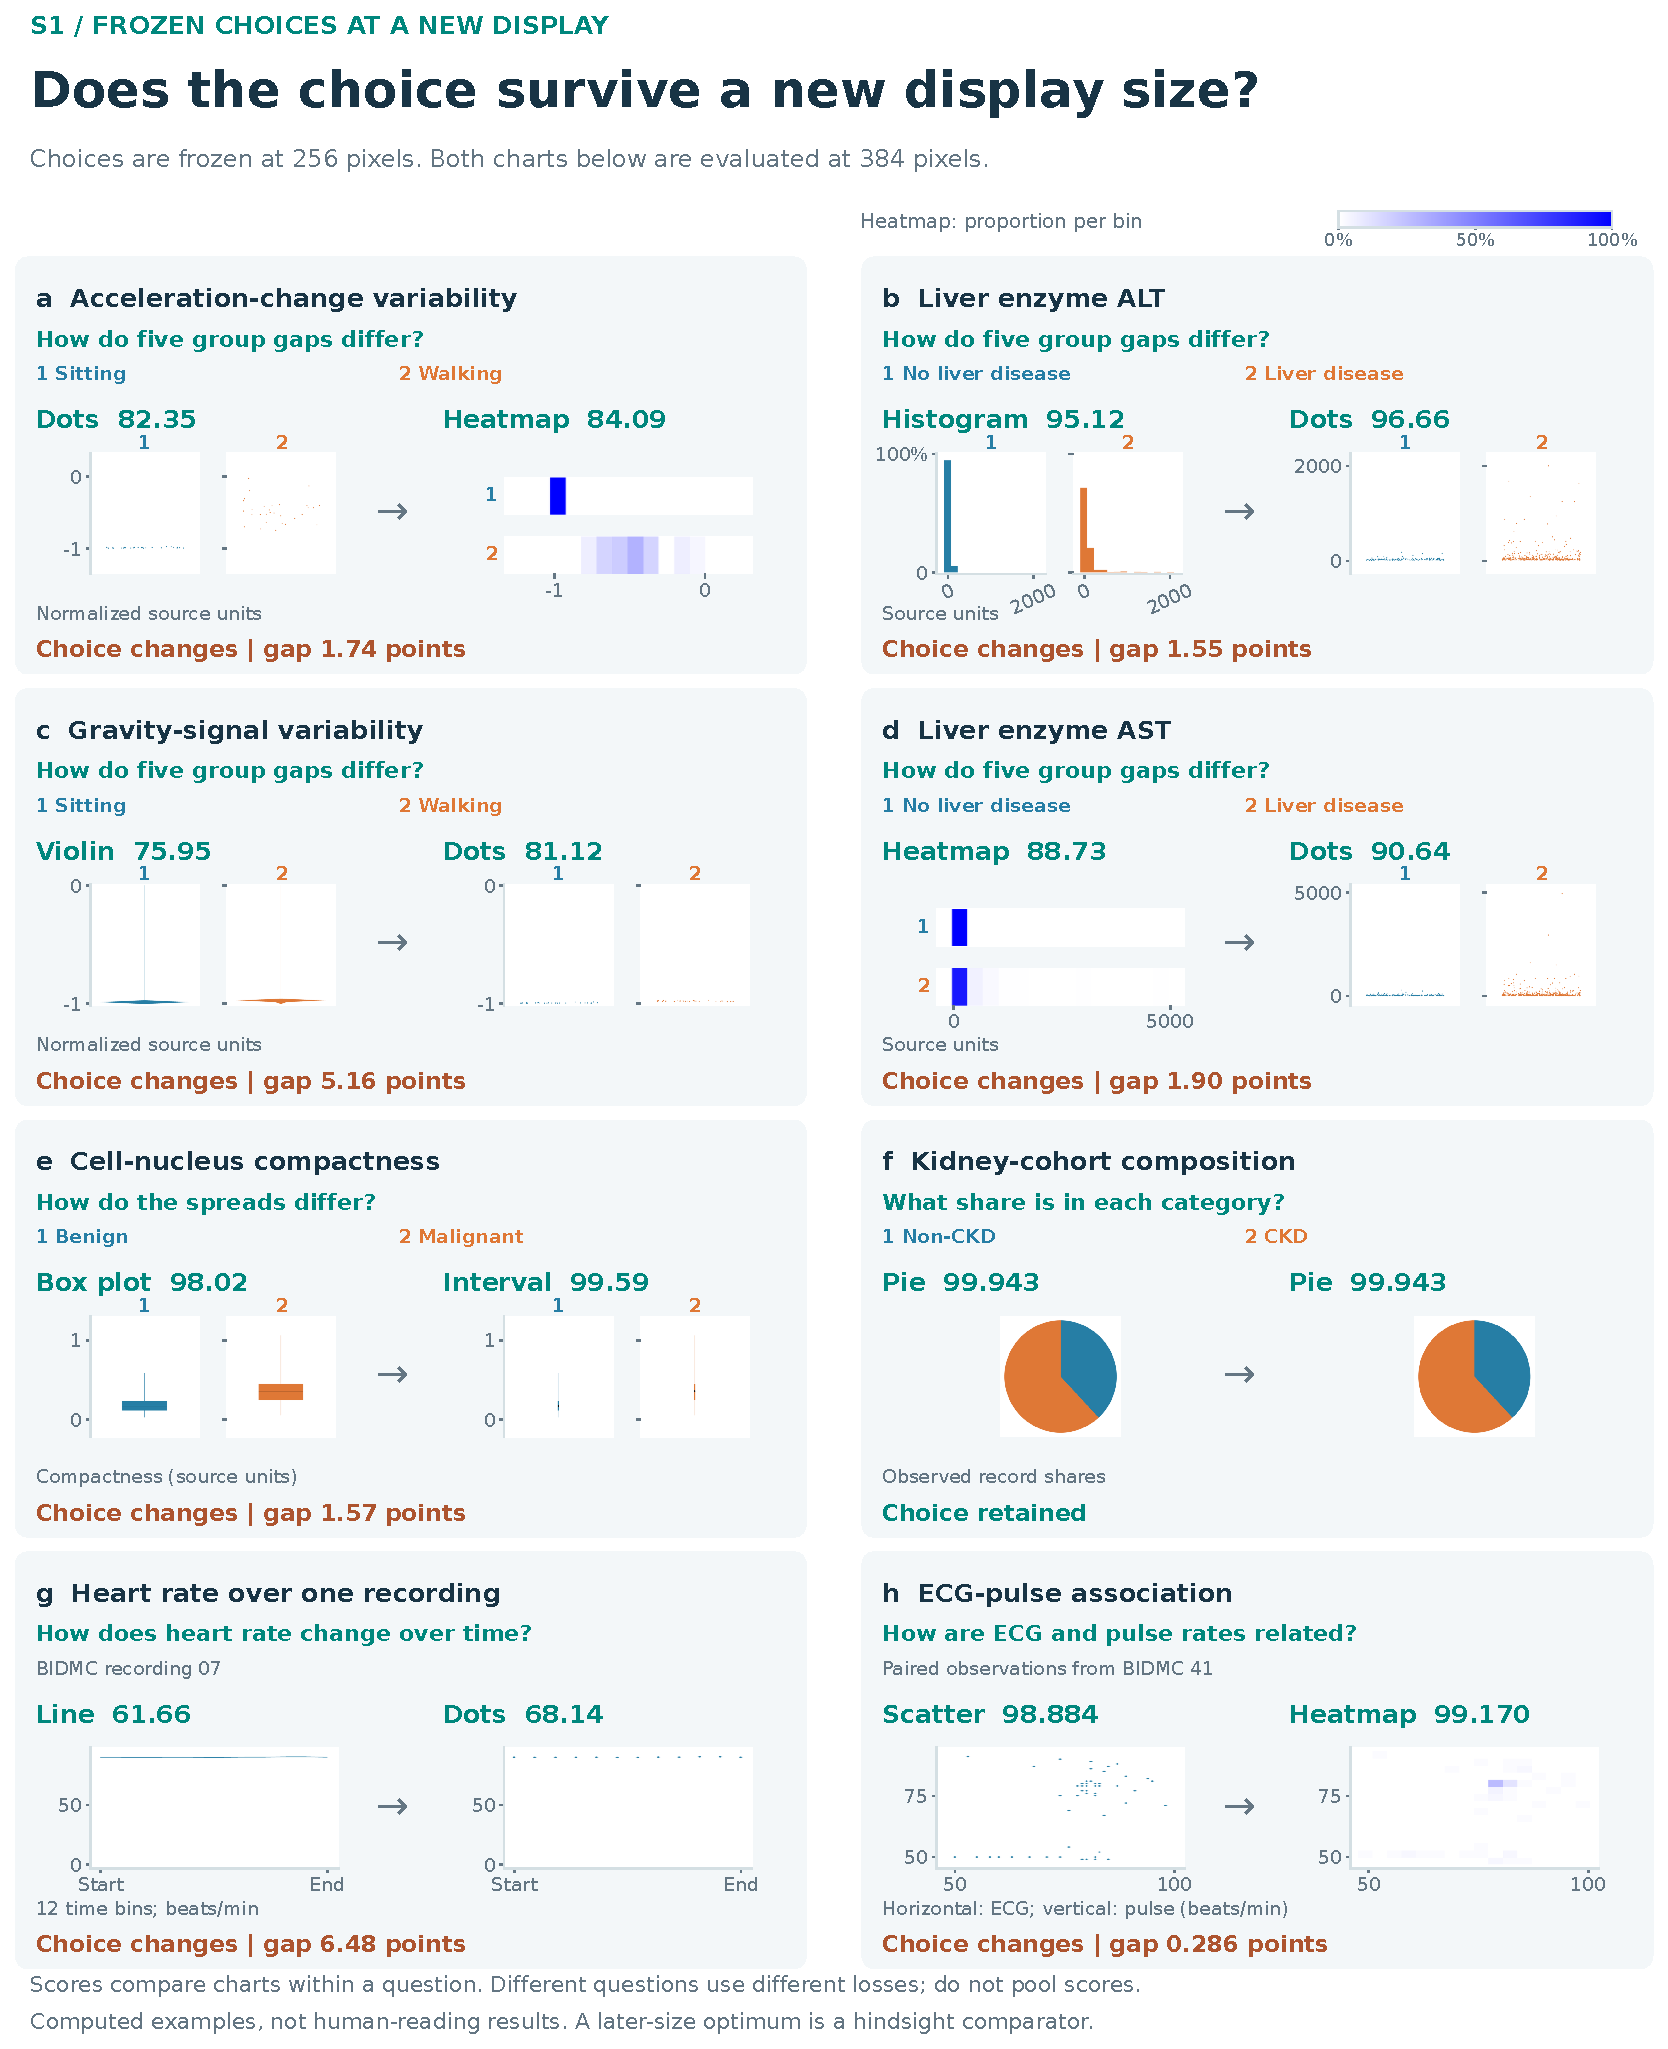
\includegraphics[width=\linewidth,height=.83\textheight,keepaspectratio]{reader_figures/figures/Figure_3_When_optimization_does_not_help.pdf}
\caption{\textbf{Deliberately selected transfer examples.} For each illustrated family/task pair, the case with the largest deficit against the later-display optimum is shown. Both scores use the later display. Seven illustrated choices change and one remains best. These are selected examples of sensitivity, not its prevalence or a causal isolation of resolution.}
\end{figure}
\clearpage
\begin{figure}[p]\centering
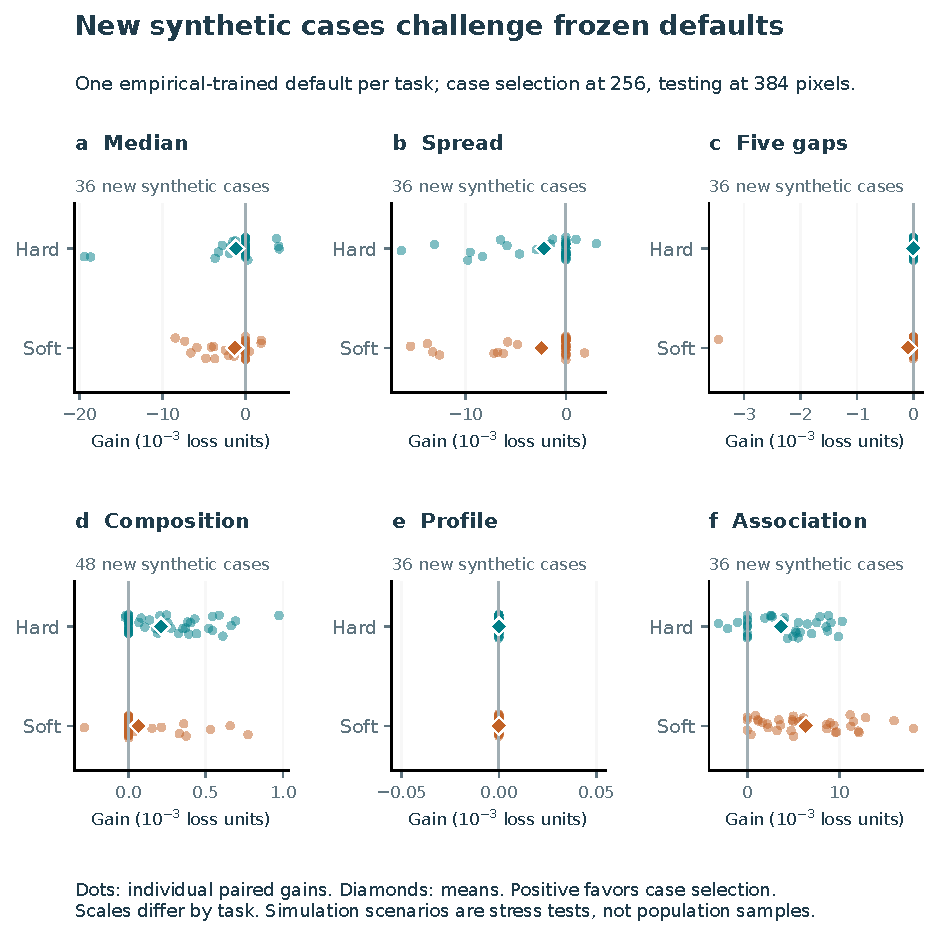
\includegraphics[width=\linewidth]{benchmark_release/figures/Figure_S3_Synthetic_detail.pdf}
\caption{\textbf{Magnitude of gains and losses on every new synthetic case.} This complements the case counts in main Figure 6. Each dot is default error minus selected-chart error for one case; diamonds are means. Positive values favor selection and negative values favor the default. Hard and soft are the algorithms called Reader 1 and Reader 2 in the main figures. Each panel has its own task-specific loss scale, multiplied by 1,000. Visual jitter separates overlapping points and is unrelated to rendering placements. Defaults were frozen from empirical data; case-specific choices use the reference display and both policies are tested on the changed display. These scenarios are a designed stress test, not a population sample.}\label{fig:synthetic-detail}
\end{figure}
\clearpage

\section*{S12. Reproduction and verification}
The final package contains raw source copies, deterministic preparation, reference arrays, all code, pinned dependency versions, saved empirical and synthetic decodes, configuration scores, trained defaults, held-out folds, case-level policy losses, failure records and SHA-256 manifests. Run \texttt{python reproduce\_benchmark.py --full} to regenerate the primary study. Run \texttt{--verify} to audit supplied results and \texttt{--figures} to rebuild the publication figures and tables. PDF compilation uses pdfLaTeX and BibTeX through the supplied build command.

Raw-source verification checks all 156 files against inherited SHA-256 hashes. The HAR source archive matches its recorded acquisition checksum exactly. The wrist reconstruction recovers 1,364 bins from 19 annotation/header pairs with maximum discrepancy $2.84\times10^{-14}$; all 149 prepared group arrays (127 primary and 22 excluded Parkinsons comparisons) reproduce exactly.

The empirical rerun reproduces 30,480 marginal candidate--task--environment aggregates and 2,728 new-task candidate--environment aggregates against the supplied earlier release within absolute tolerance $10^{-12}$, retaining missing values. Every one of the 23,808 new primary synthetic losses is independently recomputed from decoded outputs and source-array targets; maximum discrepancy is $2.22\times10^{-16}$. All 168 strong-default folds exclude their held-out resource or patient, and the 1,060 empirical case--observer policy pairs use test-display values. Checks cover blank-image rejection, target definitions, unit scaling, metadata restrictions and transfer bookkeeping.

These counts describe numerical consistency checks. They are not reader observations, independent laboratories or claims that every possible software environment gives identical pixels. The included environment pins match the tested environment. Reports distinguish regenerated primary analyses from retained historical sensitivities.

\section*{S13. Prospective reader validation: a plan, not a result}
The separate \texttt{READER\_STUDY\_PROTOCOL.md} is a plan for future work, not completed validation. It specifies new test examples, frozen selectors and defaults, counterbalanced assignment, participant and case effects, numerical estimation error, completion time and confidence. Sample size must be based on pilot variance and a prespecified meaningful effect. Ethics review, consent and recruitment have not been claimed or performed. Human results must not be inferred from synthetic data or the computational scores.

\begingroup\small\bibliographystyle{viznumbered}\bibliography{references}\endgroup
\end{document}
